\title{Data Structures - Assignment 0, Solution} 
\author{Induction and Asymptotic Notations.}
\date{September 2021}
\documentclass{article}


\usepackage[utf8]{inputenc}
\usepackage[a4paper, total={6in, 9in}]{geometry}
\usepackage{braket}
\usepackage{xcolor}
\usepackage{amsmath}
\usepackage{amsfonts}
\usepackage{tikz}
\usepackage{svg}
\usepackage{graphicx}
\usepackage{media9}
\usepackage{float}
\usetikzlibrary{calc}
\usepackage{array}
\usepackage[ruled,vlined,linesnumbered]{algorithm2e}

\usepackage[
backend=biber,
style=alphabetic,
sorting=ynt
]{biblatex}



\newcommand{\commentt}[1]{\textcolor{blue}{ \textbf{[COMMENT]} #1}}
\newcommand{\ctt}[1]{\commentt{#1}}
\newcommand{\prb}[1]{ \mathbf{Pr} \left[ {#1} \right]}
\newcommand{\onotation}[1]{\(\mathcal{O} \left( {#1}  \right) \)}
\newcommand{\ona}[1]{\onotation{#1}}
\newcommand{\nvar}[2]{ \( #1_{1}, #1_{2} ... #1_{#2}  \) }
%\newenvironment{proof}[0]{\paragraph{Proof.}}{}
%\newenvironment{remark}[0]{\textit{remark}}{}
\newenvironment{cor}[0]{\paragraph{Corollary.}}{}
\newenvironment{example}[0]{\paragraph{Example.}}{}
%\newenvironment{thm}[0]{\paragraph{Theorem.}}{}
\newtheorem{prop}{Proposition}
\newtheorem{ex}{Exercise}
\newtheorem{sol}{Solution}
\newtheorem{theorem}{Theorem} 		
\newtheorem{thm}{Theorem}[section]
\newtheorem{conj}[thm]{Conjecture} 	
\newtheorem{lemma}[thm]{Lemma}
\newtheorem{corollary}[thm]{Corollary} 
\newtheorem{claim}[thm]{Claim}
\newtheorem{proposition}[thm]{Proposition}
\newtheorem{definition}{Definition} 
\newtheorem{remark}{Remark}
 


% \addbibresource{sample.bib} %Import the bibliography file
\begin{document}    
\maketitle

\paragraph{Exercise 1. Induction.}Prove the following inequalities by induction:
\begin{enumerate}
    \item \( 2^n \le n!\) for \(n\ge 4\).
    
    \textbf{Solution.} Base, \(n=4 \Rightarrow 16\le 24\),
    
    assume that \(2^{n-1} \le (n-1)! \) for \(n\ge 5\) then we get: \[ n! = (n-1)! \cdot n \ge 2^{n-1} \cdot n \ge 2^{n-1} \cdot 2 = 2^{n} \] 
    \item \(\prod^{n}_{j=1}{\left(1 +\frac{1}{j^2}\right)} \le n+1\).
    
    \textbf{Solution.} Base, \( n = 1 \Rightarrow 1+\frac{1}{1} = 2 \le 1 + 1\) . Assume that the above holds for \(n-1\). then: \[\prod^{n}_{j=1}{\left(1 +\frac{1}{j^2}\right)} = \left(\prod^{n-1}_{j=1}{\left(1 +\frac{1}{j^2}\right)}\right) \cdot \left(1+\frac{1}{n^2}\right) \le n\left(1+\frac{1}{n^2}\right) = n + \frac{1}{n} \le n+1\]
    \item Prove that \( \displaystyle 1^3+2^3+3^3+\cdots+ n^3=\frac{n^2(n+1)^2}4 \).
    
    \textbf{Solution.} Denote by \( P(n) \) the following statement: \[ 1^3+2^3+\cdots+  n^3=\frac{n^2(n+1)^2}4.\] We can easily check that \( P(1) \) is true. This follows from the fact that \( \displaystyle P(1)\equiv\left( 1^3= \frac{1^2\cdot (1+1)^2}{4}\right) \).
Assume now that \( P(k) \) is true for some integer \( k \). We will prove that the proposition \( P(k+1) \) is true as well. We can write \begin{eqnarray*}
1^3+2^3+\cdots+ k^3+(k+1)^3&=&\left(1^3+2^3+\cdots+ k^3\right)+(k+1)^3\\
&=&\frac{k^2(k+1)^2}{4}+(k+1)^3=\frac{(k+1)^2\left(k^2+4(k+1)\right)}4\\
&=&\frac{(k+1)^2\cdot(k+2)^2}{4}.
\end{eqnarray*}


\item For a convex polygon with n sides, the number of diagonals is \(\frac{1}{2}n\left(n-3\right)\).
    \tikzset{%
      every neuron/.style={
        scale=0.2,
        circle,
        draw=black,
        fill=black,
        % maximum size=.5ex %1.5cm
      },
      neuron missing/.style={
        draw=none, 
        scale=2,
        text height=0.25cm,
        execute at begin node=\color{black}$\vdots$
      },
    }
    % \begin{center}
    
    
    \begin{tabular}{ m{5cm} m{9cm}  }
     \resizebox{150}{150}{
    \begin{tikzpicture}
    % \draw{}
    \foreach \y [count=\yi] in {-1,-0.7,0,0.7,1}  
        \node [ every neuron ] (pointu-\yi) at (\y,{sqrt(1-\y*\y)}) {};
        % \draw[black,fill=black] (\y,{sqrt(1-\y*\y)}) circle (.5ex);
    \foreach \y [count=\yi] in {-1,-0.7,0,0.7,1} 
        \node [ every neuron ] (pointd-\yi) at (\y,{-sqrt(1-\y*\y)}) {};
    \foreach \y [count=\yi] in {3,4,5} 
        \draw [-] (pointu-1) to (pointu-\y);
    \foreach \y [count=\yi] in {3,4,5} 
        \draw [-] (pointu-1) to (pointd-\y);
    \draw [-] (pointu-2) to (pointd-2);
    
    \foreach \y [count=\yi] in {2,3,4,5} 
        \draw [red,-] (pointu-\yi) to (pointu-\y);
    \foreach \y [count=\yi] in {2,3,4,5} 
        \draw [red,-] (pointd-\yi) to (pointd-\y);
    
    \end{tikzpicture}} & \textbf{Solution.} For the base consider triangle, which hasn't diagonals. That case matches the formula where \(n=3\Rightarrow \frac{3\cdot(3-3)}{2}\). Assume the rightness of the claim for every convex polygon with less then \(n-1\) sides, and consider a \(n\)-sides convex polygon. Now, fix a point, and pass \(n-3\) diagonals from it to the \(n-3\) other points. Then pass a crossing diagonal between it's two adjacent vertices. The convex property guarantees that the last diagonal we have draw divides the polygon into a left triangle and right \(n-1\) convex polygon. By applying the assumption we count an \[ (n-3) + 1 + \frac{(n-1)(n-4)}{2} =\frac{1}{2}n(n-3) \]   \\  
    \end{tabular}
    % \end{center}
    
    
    \item For a binary tree (not necessarily complete) of height \(h\), the number of nodes is less then \(2^{h+1} -1 \).
    
    
    \textbf{Solution.} Base, in the case \(h = 0\) the tree include only single node, and the number of nodes indeed equal to \(2^1  -1 = 1\). Assume the inequality hold for height \(h-1\). Consider the arbitrary binary tree of height \(h\). Notice, That the number of nodes is the sum of the root, and the nodes which are descendants of the left and the right child's of the root. Each root's child lay out a separate binary tree of height \(h-1\). So by in total we get: #nodes \(=\) \#root \(+\) \#left \(+\) \#right \(\le 1 + 2 \cdot \left(2^{h} -1\right) = 2^h - 1 \).       
    
    
    \item  Prove that for every positive integer \( n \) there exist positive numbers \( a_{11} \),  \( a_{21} \), \( a_{22} \), \( a_{31} \), \( a_{32} \), \( a_{33} \), \( \dots \), \( a_{n1} \), \( a_{n2} \), \( \dots \), \( a_{nn} \) such that 
\[ a_{11}^2=a_{21}^2+a_{22}^2=a_{31}^2+a_{32}^2+a_{33}^2=\cdots=a_{n1}^2+\cdots+a_{nn}^2.\]
    
    
    \textbf{Solution.}  Induction on \( n \):
The statement holds for \( n=1 \). Assume that it holds for some \( n \) and let us prove it for \( n+1 \). 
Assume that \( a_{11} \), \( \dots \), \( a_{nn} \) are the numbers satisfying 
\[ a_{11}^2=a_{21}^2+a_{22}^2=a_{31}^2+a_{32}^2+a_{33}^2=\cdots=a_{n1}^2+\cdots+a_{nn}^2.\]
Let us define \( a_{i,j}^{\prime}=a_{i,j} \) for \( i\leq n+1 \) and \(j < n\); define
\( a^{\prime}_{n+1,n}=a^{\prime}_{n+1,n+1}=\frac{a_{n,n}}{\sqrt{2}} \). 
Then the relations hold for numbers \( a^{\prime}_{11}, a^{\prime}_{21},a^{\prime}_{22},\dots, a^{\prime}_{n+1,n+1} \) as \[ \sum^{n+1}_{j=1}{a^{\prime 2}_{n+1,j}} = \left(\sum^{n-1}_{j=1}{a^{\prime 2}_{n+1,j}} \right) + a^{\prime 2}_{n+1,n} + a^{\prime 2}_{n,n+1} = \sum^{n}_{j=1}{a^{2}_{n+1,j}} = \sum^{n}_{j=1}{a^{2\prime}_{n,j}} \].


% ------ FOR THE NEXT YEAR ---------%
%     \item (harder version where the \(a_i\) are strict to be integers)  Prove that for every positive integer \( n \) there exist positive integers \( a_{11} \),  \( a_{21} \), \( a_{22} \), \( a_{31} \), \( a_{32} \), \( a_{33} \), \( \dots \), \( a_{n1} \), \( a_{n2} \), \( \dots \), \( a_{nn} \) such that 
% \[ a_{11}^2=a_{21}^2+a_{22}^2=a_{31}^2+a_{32}^2+a_{33}^2=\cdots=a_{n1}^2+\cdots+a_{nn}^2.\]
    
%     \textbf{Solution.}  Induction on \( n \):
% The statement holds for \( n=1 \). Assume that it holds for some \( n \) and let us prove it for \( n+1 \). 
% Assume that \( a_{11} \), \( \dots \), \( a_{nn} \) are the numbers satisfying 
% \[ a_{11}^2=a_{21}^2+a_{22}^2=a_{31}^2+a_{32}^2+a_{33}^2=\cdots=a_{n1}^2+\cdots+a_{nn}^2.\]
% Let us define \( a_{ij}^{\prime}=5a_{ij} \) for \( 1\leq j\leq i\leq n \). Let us define
% \( a^{\prime}_{n+1,i}=3a_{n,i} \) for \( 1\leq i\leq n \), and \( a^{\prime}_{n+1,n+1}=4a_{11} \). 
% Then the relations hold for numbers \( a^{\prime}_{11}, a^{\prime}_{21},a^{\prime}_{22},\dots, a^{\prime}_{n+1,n+1} \).
% -------------------------------- %

\end{enumerate}

\paragraph{Exercise 2. O-notation.}
\begin{enumerate}
\item Prove that \(2^{\sqrt{n}} = \Omega\left(n^k\right)\) for every \(k \in \mathbb{R}^{+}\). 

 \textbf{Solution.} By induction, we will prove that there exists \(c >1\), and \(n_0\) such that for every \( n > n_0\) it's hold that: \(2^{\sqrt{n}} > cn^k\), for the base case consider \(n_0 = k^{10}\), and extract \(\log\) from both sides, which become \( k^5 \ge 10k\log k\). It is clear there exists such a \(c\) (which is \(k\) depended, for example if \(k \ge 1 \) then \( c \le 10 \)). Assume the rightness of the claim for every \(n^\prime < 2n\). Thus: \begin{equation*}
 \begin{split}
     2^{\sqrt{2n}} &= 2^{\sqrt{2}\sqrt{n}} = \left( 2^{\sqrt{n}}\right)^{\sqrt{2}} \ge \left(cn^{k} \right)^{\sqrt{2}} \ge c\left(n^{\sqrt{2}}\right)^{k}
      \end{split}
 \end{equation*}
 By the fact that \( n^{\sqrt{2}} \ge n\cdot n^\frac{1}{10} > 2n \) for every \(n \ge 100 \) we get: 
 \begin{equation*}
 \begin{split}
      c\left(n^{\sqrt{2}}\right)^{k} > c\left(2n\right)^{k} 
      \end{split}
 \end{equation*}
The same calculation leads to \(2^{\sqrt{2n+1}} > c\left(2n+1\right)^{k}\) and that finishes the proof. 

\item Prove that for every pair of functions \(f,g : \mathbb{N} \rightarrow \mathbb{R}^{+}\) \begin{equation*}
     O \left( f + g \right) = O \left( \max{\{f,g\}} \right)
\end{equation*} 

 \textbf{Solution.} Let \(n\) be an integer \(n \in \mathbb{N}\), and suppose without loss of generality that \(f(n) > g(n)\) (if the opposite occurs then swap the functions names). Therefore   \begin{equation*}
 \begin{split}
     f(n) + g(n) \le f(n) + f(n) \le 2f(n) = 2 \max{\{f(n), g(n)\}}
      \end{split}
 \end{equation*}
That it, for every \(n \in \mathbb{N}\) the summing is bounded by \( 2 \max{\{f(n), g(n)\}} \Rightarrow f(n) + g(n) = O\left(\max{\{f(n), g(n)\}}\right)\).

\item Let \(\zeta_r\) be the area of \(r\)-radius circle. Define a \textit{tiling} as set of non overlapping rectangles with unit-length side such that each rectangle is inside the circle (and doesn't cross the border). Define \(\eta_r\) to be the maximum area of \(r\)-radius circle tiling, Prove that \( \zeta_r = \Theta\left(\eta_r\right)\).  

    \tikzset{%
      every neuron/.style={
        scale=0.2,
        circle,
        draw=black,
        fill=black,
        % maximum size=.5ex %1.5cm
      },
      neuron missing/.style={
        draw=none, 
        scale=2,
        text height=0.25cm,
        execute at begin node=\color{black}$\vdots$
      },
    }
\begin{tabular}{ m{5cm} m{9cm}  }
     \resizebox{150}{150}{
    % \usetikzlibrary{calc}
    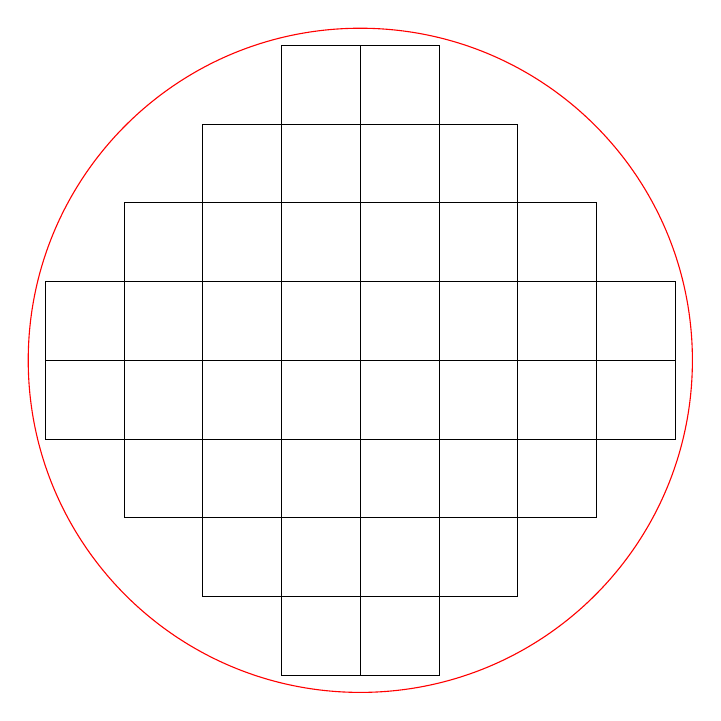
\begin{tikzpicture}
    % \usetikzlibrary{abs}
    \foreach \y [count=\yi] in { 0,1,...,4 }  {
        \foreach \x [count=\xi] in {0,1,...,4}{  %}%,0,0.2}%,0.4,0.6,0.8,1} 
        \pgfmathtruncatemacro{\r}{ \x + \y};
            \ifthenelse { \r < 4 } {
            \draw[draw=black] (\x,\y) rectangle ++(1,1);
            \draw[draw=black] (\x,-\y) rectangle ++(1,-1);
            \draw[draw=black] (-\x,\y) rectangle ++(-1,1);
            \draw[draw=black] (-\x,-\y) rectangle ++(-1,-1);
            } {};
        };
    };
    \draw[red](0,0) circle (120pt);
    % \draw[draw=black] (0,0.2) rectangle ++(0.2,0.2);
    %     \node [ every neuron ] (pointu-\yi-\xi) at (\x,\y)) {};
    %     % \draw[black,fill=black] (\y,{sqrt(1-\y*\y)}) circle (.5ex);
        % \node [ every neuron ] (pointd-\yi) at (\y,{-sqrt(1-\y*\y)}) {};
    % \foreach \y [count=\yi] in {3,4,5} 
    %     \draw [-] (pointu-1) to (pointu-\y);
    % \foreach \y [count=\yi] in {3,4,5} 
        % \draw [-] (pointu-1) to (pointd-\y);
    % \draw [-] (pointu-2) to (pointd-2);
    
    % \foreach \y [count=\yi] in {2,3,4,5} 
    %     \draw [red,-] (pointu-\yi) to (pointu-\y);
    % \foreach \y [count=\yi] in {2,3,4,5} 
    %     \draw [red,-] (pointd-\yi) to (pointd-\y);
    
    \end{tikzpicture}} & \textbf{Solution.} By the definition of tiling the upper bound \(\eta_r = O\left(\zeta_r\right)\) follows immediately. It has left to bound \(\eta_r\) from below. Notice that the maximum tiling area is greater (by been a maximum) then the configuration in which we fill the lattice (table) \([-r, r] \times [-r, r]\) such that the points \( \{ (x,y),(x+1,y),(x+1,y+1), (x,y+1) \} \) are the vertices of rectangle only if it doesn't get outside of circle. Call for that tiling, a \textit{bin packing}. Thus:
    
    \end{tabular}
    \begin{equation*}
        \begin{split} \eta_r & \ge S(\mathbf{bin\ packing})= 2\lfloor r \rfloor + 2\cdot\sum_{i=0}^{\lfloor r \rfloor}{2\lfloor r - i \rfloor} \ge 
            2\lfloor r \rfloor + 2\cdot\sum_{i=0}^{\lfloor r \rfloor}{2\lfloor r \rfloor - \lceil i \rceil } = \\ & 4 \lfloor r \rfloor^2 + 2\lfloor r \rfloor  - \frac{1}{2}\left( \lfloor r \rfloor \right)\left(\lfloor r \rfloor - 1\right) \ge \frac{1}{100} \frac{1}{2} \pi r^2 \ \ \ (\mathbf{for\ } r > 2)
        \end{split}
    \end{equation*}
    Therefore we conclude that \(\eta_r = \Theta(\zeta_r) \).

\end{enumerate}
% \paragraph{Exercise 2. Hierarchy Collapsing.}Let assume the following false statement,  suppose there exists an index \(k \in \mathbb{N}\) such that \(n^k = \Theta\left(n^{k+1}\right) \). 
% \begin{enumerate}
%     \item show that growth of arbitrary polynomial of degree \(d\) is bounded by constant  \( n^d = \Theta \left(1 \right)  \)
%     \item show that the above holds also for exponential growth, \( 2^n = \Theta \left(1 \right)  \)
% \end{enumerate}

% \paragraph{Solution.}

% \paragraph{Exercise 3. Arithmetic Mean Behavior.}Prove or disprove,  Let \(f:\mathbb{N} \rightarrow \mathbb{R}^{+}\) be a function such that: \( f(n) = \Theta\left(\frac{1}{n}\sum^{n}_{i=1}{f(i)}\right)\), let \(M\) be a set of \(log\left(n\right)\) arbitrary points, in the range \( \{1,2...,n\}\).

% Does the following bound hold? \begin{equation*} 
%     f(n) = \Theta\left(\frac{1}{n}\sum^{n}_{i=1, i\notin M }{f(i)}\right)
% \end{equation*} 


% \paragraph{Solution.}By the fact that big-\(\Theta\) define equivalence class, It is enough to prove that  \begin{equation*} \overbrace{\frac{1}{n}\sum^{n}_{i=1, i\notin M }{f(i)}}^A = \overbrace{\Theta\left(\frac{1}{n}\sum^{n}_{i=1}{f(i)}\right)}^{B}\end{equation*}. As \(f\) mapping only to positive numbers, the upper bound \(A = O(B)\) steams immediately. Thus, it is left to show that \(A = \Omega(B)\). Notice that \(A = B - \frac{1}{n}\sum_{i\in M}{f(i)}\ge B - \frac{\log(n)}{n}\max_{i\in M}{f(i)} \). The given property \( f(n) = \Theta\left(\frac{1}{n}\sum^{n}_{i=1}{f(i)}\right)\) yields that there exists number \(c > 0\) such that: \begin{equation*}
%     B - \frac{\log(n)}{n}\max_{i\in M}{f(i)} \ge B -\frac{c\cdot\log(n)}{n}\frac{1}{i}\sum_{j}^{i\leftarrow arg\max M}{f(j)}
% \end{equation*}     


% \printbibliography 
\end{document}
